\subsection{Opsamling og behandling af EMG-signaler} \label{sec:EMG_imp}
For at opfylde de krav, der er opstillet i \autoref{sec:EMG_krav} anvendes Muscle Sensor V3 fra Advancer Technologies, der fremover vil refereres til som 'EMG-forstærker'. Denne komponent måler en differens mellem de elektriske potentialer, der måles gennem elektroderne. EMG-forstærkeren overholder de opstillede krav, og kan anvendes direkte med mikrokontrolleren. EMG-forstærkeren består af en intrumenteringsforstærker, et passivt højpasfilter, en full-wave rectifier, et aktivt lavpasfilter og en justerbar forstærker \citep{advancertech2013}. 

En illustration af, hvordan EMG-forstærkeren behandler et inputsignal fremgår af \autoref{fig:sinussignal}.
\begin{figure}[H]
\centering
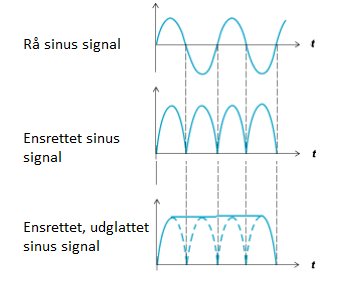
\includegraphics[width=0.6\textwidth]{figures/sinussignal.png}
\caption{Tre sinussignaler. Henholdsvis et råt, ensrettet og ensrettet samt udglattet. \citep{advancertech2013}.}
\label{fig:sinussignal}
\end{figure}

\noindent
På \autoref{fig:sinussignal} kan sinuskurven opfattes som muskelsignalet. Dette passerer et passivt højpasfilter bestående af en kondensator, der dæmper DC-støjen og dermed offsettet i signalet. Dette betyder, at muskelsignalet centeres omkring 0 på tids-aksen, hvilket er nødvendigt for at få ensretningen til at virke efter hensigten, da ensretningen foregår omkring denne akse. Dernæst helbølgeensrettes signalet på midterste graf, ved at invertere signalets negative værdier, så signalet udelukkende består af positive værdier samtidigt med at beholde hele dets originale energi. Herefter envelopefiltreres signalet, hvilket ses som det udglattede signal på nederste graf. Til denne filtrering er der beregnet en knækfrekvens på $1,94~Hz$ ud fra \autoref{eq:lavcutfre}. $C$ og $R$ kan i databladet for EMG-forstærkeren aflæses til at være henholdsvis $1 \cdot 10^{-6}~F$ og $80,6 \cdot 10^3~\Omega$ \citep{advancertech2013}. 

\begin{equation}\label{eq:lavcutfre}
f_c = \frac{1}{2 \pi C R} = \frac{1}{2 \pi \cdot 1 \cdot 10^{-6}~F \cdot 80,6 \cdot 10^3~\Omega} = 1,94~Hz
\end{equation}

\noindent
Ud over ovennævnte kræver EMG-forstærkeren en spændingsforsyning på minimum $\pm 3~V$ og maksimalt $\pm 30~V$. Herudover er der mulighed for at justere modstanden fra $0,1~\Omega$ til $100~k\Omega$, hvilket giver et justerbart gain fra 0,002 til 20.700 gange. \citep{advancertech2013}. 